\chapter*{"Ubersicht}
\begin{refsection}
Im zweiten Teil werden Anwendungsbeispiele aus der HPC-Welt gezeigt.
Eigentliche rechnerische L"osungen stehen hier neben mathematischen
"Uberlegungen, wie man ein Problem der L"osung mit leistungsf"ahiger
Rechnerhardware zug"anglich macht.

{\em Marco Bassotti} und {\em Dario Tr"utsch} verwenden OpenCL,
um die R"uckprojektion zur Radon-Transformation
auf paralleler Hardware zu berechnen, sie erreichen dabei eine erstaunliche
Beschleunigung der Rechnung.
Die R"uckprojektion ist ein wesentlicher Schritt, um mit einem
Computertomographen aus den Rohdaten Bilder entstehen zu lassen.

{\em Nicol\'as Rom\'an L"uthold} und {\em Flavio La Morea}
wagen sich an das Problem,
einen Kugelsternhaufen zu simulieren. Das Problem ist nicht einfach,
w"achst doch der Simulationsaufwand mit der dritten Potenz der Anzahl
der Sterne.
Es gelingt ihnen, trotz dieser widrigen Umst"ande, ein Video der Dynamik
eines kleinen Sternhaufens zu erstellen.

{\em Danilo Bargen} und {\em Lukas Murer} lassen die geballte Rechenleistung von GPUs
mit Hilfe von OpenCL auf das Problem los, Passwort-Hashes zu knacken.
Ihre Rechenbeispiele zagen, wie Passwort-Hashes von Passw"ortern mit nur
6 Stellen innert Sekunden geknackt werden k"onnen.

{\em Tabea M\'endez} und {\em Christian Schmid} f"uhren die Berechnung des aus der
Theorie der komplexen dynamischen Systeme bekannten ``Apfelm"annchens''
in Quaternionen durch. Da die Quaternionen einen vierdimensionalen
Raum bilden, w"achst die Datenflut bei Steigerung der Aufl"osung mit
der vierten Potenz an, und auch die Visualisierung dieser grossen Datenmengen
ist nicht trivial.

{\em Gregor Dengler} hat sich mit OpenFOAM, einem Open Source
System zur L"osung partieller Differentialgleichungen befasst, und berichtet
"uber dessen Nutzen, aber auch "uber die speziellen Schwierigkeiten,
die man mit so einem Produkt treffen kann.

{\em Dorian Amiet} und {\em Hannes Badertscher} haben Experimente mit
Monte Carlo Simulationen gemacht, und sind beim Einsatz von OpenCL auf
einige spezielle Schwierigkeiten gestossen. Sie untersuchen vor allem auch
das Problem, wie man Zufallszahlen ausreichend hoher Qualit"at f"ur 
solche Simulationen in einer OpenCL Anwendung bekommen kann.

{\em Daniel Monti} und {\em Pascal Stump} haben versucht, das Konzept
von Map-Reduce auf die Berechnung des Eigenvektors zum Eigenwert $1$
einer Wahrscheinlichkeitsmatrix zu adaptieren. Sie haben dazu eine eigene,
parallelisierbare Version des Potenzalgorithmus gefunden.

{\em Felix Hofer} zeigt, wie Successive Overrelaxation die
Konvergenz eines iterativen Verfahrens zur L"osung linearer Gleichungen
verbessern kann.

{\em Reto Christen} und {\em Philipp Solenthaler} l"osen das Potentialproblem
mit OpenMPI. Sie untersuchen, wie sich der bestehende Code f"ur das
W"armeleitungsproblem, welcher nur das Jacobi-Verfahren unterst"utzt,
auf die Verwendung des Gauss-Seidel-Algorithmus erweitern l"asst, und
wie sich dies auf die Laufzeit auswirkt.

{\em Andreas Linggi} und {\em Stefan Steiner} wenden die L"osung des
Potentialproblems auf eine Visualisierung der Greenschen Funktion an.

{\em Fabian Klein} und {\em Thomas Ziegler} wagen sich an die numerische
L"osung der Gleichung von Burgers. Als Prototyp einer nicht linearen
partiellen Differentialgleichung, die nahe verwandt ist mit den
Str"omungsgleichungen, l"asst sich aus deren L"osung viel "uber "ahnliche
Modelle zum Beispiel in der numerischen Wetterprognose lernen.

Damit schliesst sich der Kreis der Awendungen. Lewis Fry Richardson hat
sich vor ziemlich genau hundert Jahren eine Methode zur Berechnung der
Wetterentwicklung ausgedacht \cite{skript:richardson}.
Zu deren Durchf"uhrung stellte er sich
eine {\em Forecast Fatory} vor (Abbildung~\ref{forecastfactory}),
ein riesiges, theaterartiges Geb"aude,
wo viele Computer, also Arbeiter mit mechanischen Rechenmaschinen an der
Berechnung der Atmosph"arenentwicklung f"ur jeweils ein Teilgebiet
der Erdoberfl"ache arbeiten,
und ihre Resultate an ihre Nachbar-Rechner weitergeben. 
Man kann also durchaus sagen, dass Richardson der erste war, der die Vision
eines massiv parallelen Rechners zur L"osung eines HPC Problems hatte,
wenngleich mit anderer ``Technologie'' als unsere heutigen HPC Cluster.

\begin{figure}
\begin{center}
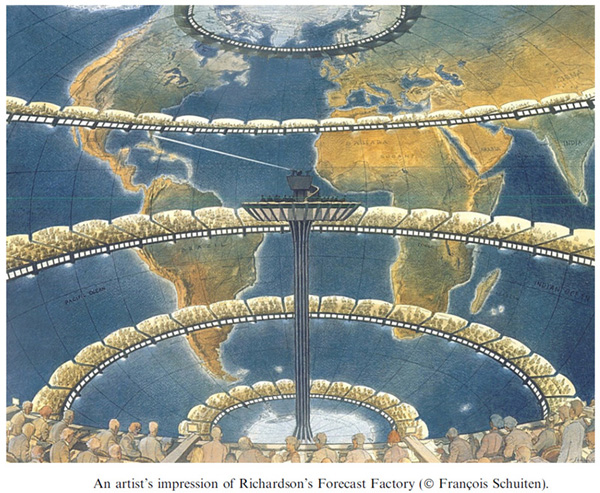
\includegraphics[width=\hsize]{images/forecast-factory-color.jpg}
\end{center}
\caption{Von Lewis Fry Richardson erdachte Vision einer Forecast-Factory
\label{forecastfactory}}
\end{figure}

\printbibliography[heading=subbibliography]
\end{refsection}
